\documentclass[5pt]{article}
\usepackage[utf8]{inputenc}
\usepackage{natbib}
\usepackage{graphicx}
\usepackage[margin=1.2in]{geometry}
\usepackage{listings}
\usepackage{titling}

\geometry{
  left = 22.5mm,
  right = 22.5mm,
  top = 20mm,
  bottom = 30mm
}


\setlength{\droptitle}{-2em}

\begin{document}
\title{WACC Compiler - Final Report - Group 29}
\date{}
\author{
Kristina Atanasova (ka4518) \\
Mohammad Ghusharib Chohan (mgc18) \\
Maksymilian Graczyk (mg5418) \\
Radina Milenkova (rm4318)
}
\maketitle

\section{Final Product}

At the end of the WACC Project, we have a fully working compiler for ARM, which passes all tests on LabTS. Also, we have tested all the advanced testfiles, as well as some of our tests including extra features we added to WACC during the extensions stage. As a result, we have completely realised the specified functionality of WACC. All of these are regularly tested on the pipeline.
\\ \\
Our compiler performs exceptionally well due to limited stages and avoiding repetition. As can be seen in the system diagram, we have broken the compiler down into a few major stages, during which only the necessary steps are carried out. The use of visitor patterns minimises the need for extensive checking and allows for a recursive generation, which ensures each kind of ASTNode carries out its necessary work and delegates extra work to the subnodes it consists of. In addition, there is no repeated computation, as any useful information is stored and remembered - a key example is type information, which is remembered inside the symbol table created in Semantic Analysis and passed through to Code Generation. Separation of Semantic Analysis into Expression Types and actual Semantic Checking also improves performance through delegation.
\\ \\
Finally, the extensions add very few stages and as a result, maintain the performance of our compiler. Optimisations (if requested) are carried out in a stage before code generation and use just one extra visitor. As optimisations largely work on simplification of ASTNodes, the ASTree is simplified and so fewer nodes need to be visited during Code Generation. A translation layer is added to translate according to the architecture but is an essential stage for cross-compiling.
\\ \\
Our compiler is written in a way that it is has a very solid base for future development. Due to the use of ANTLR, the Grammar is split into two .g4 files, one for the Lexer, one for the Parser and so it the grammar can be extended easily. The compiler is split into clear stages and packages (AST, Optimisations, Semantic Analysis...) and so it is clear to a future developer where code has been written for specific sections. In addition, the code is very well commented and explained, to ensure understanding of any individual section of code. Finally, as part of one of the extensions, we have added a translation layer. This is to hopefully simplify Code Generation for compilation into different Assembly Instruction sets e.g. x86. All in all, it forms a very sound basis for the future and it will not be difficult to continue adding features.

\section{Project Management}
For this project, we chose to adopt feature branches and rebasing as used in industry. Unlike previous projects, we did not create one branch for each member of the group. Instead, we chose branch names which described the current feature being worked on in that branch. As such, every branch and merge would be adding a new feature to master. Due to our feature-specific workflow, the strategy was clear - we would commit often and once ready to merge (feature complete), we rebase the feature branch off of master, replaying changes on top of master. As such, this is a new feature being added to the already existing solid code on master. It would get the latest changes to our WACC repository and re-test to ensure everything works well together as a whole product.
\\ \\
As a result, we did not suffer the consequences of leaving merging too late. Our features were small in size meaning it was very rare for our feature branches to live longer than 2 days, and they would be merged into master often upon completion. We always had a working implementation ready to be submitted and were rarely in a broken state on the master branch. Typically, the same people would work on one feature branch, with work being distributed between either threes, pairs or individuals in parallel.
\\ \\
To aid with this workflow, we adopted a few features of git. Firstly, we protected the master branch. This ensured that no one was allowed to push or make changes to the master branch. In addition, we used the merge requests section of GitLab for making merge requests, which would only merge into master upon a successful pipeline. Also, we made use of git squashing, where we had too many commits, to squash them into fewer, more useful commits.
\\ \\
Our pipeline was a simple 3 stage pipeline - building ANTLR, building Java files and finally testing. The testing stage has multiple jobs, one per test suite, allowing us to see which specific test suite we failed.
\\ \\
Thanks to this workflow, we had a clear end-goal all the time, making us very efficient. Splitting tasks into smaller features and assigning them to different members allowed us to work quickly and with a clear mindset about what had to be accomplished without worrying about other features. In addition, rebasing allowed us to avoid merge conflicts and conflict-related commit messages on our graph, creating a clear and useful graph at the end of the project. Rebasing allowed us to carry out work with minimal merge conflict, meaning we could spend more time writing code and less time fixing such errors.
\\ \\
However, there were a few issues in our management which could be addressed. Firstly, when merge conflicts did occur, rebasing would create a far messier merge conflict than simple merging. This was due to multiple members working on the same file, causing more than just a simple two way merge conflict which occurs with the merge command. Also, refactor stages were done as whole features, which is bad for git blame and understanding when code was changed. Next time, it would be better to refactor at the end of a feature branch before merging, instead of having whole refactor stages.

\section{Design Choices and Implementation}
\subsection{Tool-Set}
For our project, we chose to use Java alongside the ANTLR toolset. This choice was made, because Java is a language that all members were confident with, and one that we have the most experience in. As a result, we knew of all debugging tactics especially within the IntelliJ IDE, and the various features of Java we could take advantage of (e.g. Actual and Apparent Types). ANTLR was chosen as it is the suggested and most powerful Parser Tool that works with Java, and is well documented both online and in book form. We were able to easily pick up ANTLR despite never having worked with it before.
\\ \\
In addition, our choices led us to use a Gradle set up. Gradle is the simplest way to create a build tool, without having to do any major prior set-up. All we had to do was follow the specified structure for a Gradle project and as a result, we were able to generate a powerful build tool which worked straight away. Also, as a result, our Makefile could simply invoke the relevant Gradle commands. This further led us to use JUnit testing throughout the WACC Project, as the Gradle support for JUnit is strong. JUnit makes use of Parameterised unit tests which allowed us to avoid having to write individual tests for the many (over 100) test files that were provided along with our own, as well as run them in parallel on the pipeline. Also, writing test suites was faster and simpler and we were able to test many of the components of our WACC Compiler. Our compile script was a simple shell script, as the only necessary step was to invoke our main Java method in the Compiler Class.
\subsection{Compilation Stages}
The first step of the compiler uses the ANTLR powered parser to perform lexical analysis and parsing of the .wacc file. This uses the WACCLexer.g4 and WACCParser.g4 files we wrote. The next step was to generate an Abstract Syntax Tree. This was carried out before Semantic Analysis so that we could use our visitor methods inside the semantic checking, as well as simplify the process. We overcome the issue of ensuring functions have return statements by enforcing the rule inside the WACC Grammar, and so ensuring the same ASTNode was generated regardless of how a function returns was imperative to avoid code duplication.
\\ \\
The next step is Semantic Analysis, which makes use of the ASTVisitor pattern (discussed later). It determines the type of expressions by using a GetExpressionTypeVisitor and stores the information in a symbol table to avoid having to carry out type checks again in later stages. The final step is Code Generation, where an internal assembly format is generated and translated to the correct architecture before being printed out to a .s file. In the extension stage, an Optimisation step is added before Code Generation where AST Nodes are modified through optimisations. Please see Figure 1 for reference.
\begin{figure}
    \centering
    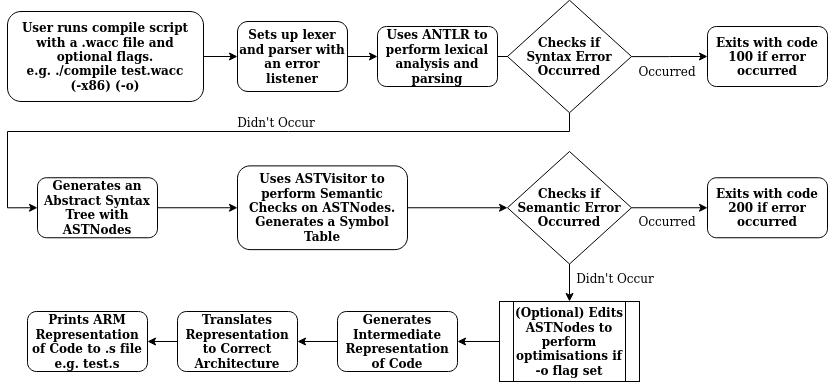
\includegraphics[width = 140mm]{SystemDiagram.png}
    \caption{A system diagram for our WACC Compiler}
    \label{fig:System Diagram}
\end{figure}{}
\subsection{Design Patterns}
Our AST Package houses the ASTNodes Classes, which makes use of interfaces and abstract classes which are a key feature of Java. This is to differentiate between Body Nodes, Expression Nodes, Assignments, Types etc. Categories of e.g. types are further enforced by the use of enums. This forces the user to use the enum values we have specified in the ASTNodes class, and cannot produce garbage or non-existent values. The use of the interface also forces every ASTNode to have a visit() method, allowing us to create a visitor pattern similar to ANTLR for our Abstract Syntax Tree. Abstract classes allow us to avoid code duplication for common Nodes such as BinaryExpressionNodes which are further broken down into individual sub-nodes such as ArithmeticNode.
\\ \\
Throughout our compiler, we continuously make use of visitor patterns. We defined an ASTVisitor interface which specifies methods for visiting all the individual nodes with a generic return type. This allows us to create various visitors which return different types. It also ensures that every visitor that is created has all the key components required to be a fully functioning visitor pattern (i.e. it does not miss out any nodes). This was a major issue that had to be overcome, which we did by having an abstract method in every node

\begin{lstlisting}
    public abstract <T> T visit(ASTVisitor<T> visitor);
\end{lstlisting}

which is over-ridden, avoiding the need for instanceof and instead depending on java calling the right method.
\\ \\
The final major design pattern used was Private Constructors with ENUMs. A major issue was ensuring developers could not have the ability to generate garbage ARM code which was fundamentally wrong. An example would be using registers which do not exist. To overcome this problem, we made use of ENUMs which were used as part of constructors. For example, to specify a register, it must be chosen from the Register ENUM, which only allows us to use r0, r1 ... LR. So in a PUSH Instruction, you can only do e.g. PUSH r0. For more complicated instructions, such as Pre Indexed Offset Registers, constructors were made private, and static methods were used instead. As a result, it is clearer to the developer what kind of instruction is being generated and what the parameters mean. An example is:
\begin{lstlisting}
    OffsetRegister.preIndexedOffset(r0, new ConstantOffset(4));
\end{lstlisting}
which easily tells us we are creating a Pre Indexed instruction of [r0, \#4]. With the extension of Cross Compiler, we added checking to enforce these rules, printing appropriate error messages if violated.
\section{Extensions}
\subsection{Bitwise Operators and Void Functions - Front End}
The lexer and parser now include ‘and’, ‘or’, eor’ and ‘shifting’ binary operators, as well as, ‘bitwise complement’ unary operator. They were added considering their precedence over the rest of the operators, so that correct associativity of all expressions is preserved. The WACC language now also supports the Void base type for functions, which was added to the lexer. Functions of that type follow the structure of the WACC return type functions, but they no longer have to end with a ‘return’ or an ‘exit’ statement.
\subsection{Advanced Generic Types (Linked Lists) - All Stages}
The WACC language was extended to support list creation of a generic type parameter. It has functions to add or remove an element from the list, as well as to check if an element is contained in the list. Printing, freeing a list and retrieving an element at a certain position are also supported. New list creation is done using the newlist() function and its size could be retrieved using listsize(). To implement those features, we made use of util methods for lists, that we created in the code generator. This includes list bounds check for throwing a runtime error upon illegal access. Tests for lists can be seen in valid/generic\_lists.
\subsection{Function Overloading - Semantic Analysis and Code Generation}
Function overloading allows us to have multiple functions with the same name but with a different number or types of arguments as well as different return types.
A new generic Function Symbol Table class was created to map string values to a list of function entries. In this way, we could associate a function name with all function declarations with this corresponding name.
At the beginning of the semantic analysis, we iterate through all function nodes and generated a function entry for each of them. Based on the function name the function entry is added to the list of function entries corresponding to that name. By associating call nodes with function entries in the symbol table, we ensure we call the correct function.
\\ \\
We associate each function entry with a function label, generating the same function label for the function node except for the additional number. This is done using the current size of the list of function entries associated with this function name. In this way, no two functions can have the same label (i.e. \_f\_1, \_f\_2, etc).
The new implementation was tested by creating new WACC test files int testfiles/valid/overloading folder. The generation of a semantic error when creating two identical functions was tested in the test files/invalid/overloading folder.
\subsection{Optimisations - Pre-Code-Generation}
We implemented 4 optimisations: Constant Evaluation, Control Flow Analysis, Constant Propagation and Removal of Unused Variables.
All four optimisations were done using an ASTBaseVisitor that visits every AST node and simplifies it if possible.

We visit the left-hand-side (lhs) and right-hand-side (rhs) of an expression node and try to get its value. This works only when the lhs and rhs are basic nodes such as IntNode, BoolNode, CharNode. If the two sides of the expression can be evaluated we return a simplified new node.
Control Flow Analysis determines the condition of an if statement and while node and retains only the relevant body if possible.

Constant Propagation is implemented by using a RememberValue visitor and a boolean field "remember" that tells you whether you know if an identifier value has possibly changed or not. When visiting an Identifier node, if we still remember the value of the identifier(the optional field of its variable declaration field is not empty) we return a simplified node(int, char, bool).

Removing unused variables was done by keeping track of the number of usages of a variable declaration. If it is equal to 0 during code generation, we do not produce assembly.

 The compile script can be run to produce optimised code with a -o flag after the file path. Test files are provided in the testfiles/valid/optimisation folder. In addition, the pipeline currently tests un-optimised and optimised code to ensure the same functionality.
 \subsection{Cross Compiler - Back End}
 One partially complete extension is the x86 cross compiler. For the purposes of this extension, an additional layer was added. After generating intermediate code, a translation layer, depending on the architecture we wish to translate to, transforms the intermediate code representation into an architecture-specific assembly. This is done by making use of a purpose built visitor pattern, similar to ASTNodes, but for Instruction classes.
 \\ \\
 To deal with the various architectures, we created interfaces and abstract classes, which the architecture-specific instructions/programs would extend. As a result, the Code Generator Visitor can perform the same task without code duplication and without considering which architecture is being used. For x86, a lot of research and subtleties of the assembly language had to be overcome and discovered during the process.
 \\ \\
Currently, we do not have full functionality of WACC for x86. The commands:
 \begin{lstlisting}
     ./compile filepath -x86
     gcc -no-pie -m32 -o filename filename.s
     ./filename
 \end{lstlisting}
 can be used to test functionality. In general, we successfully generate assembly code in x86 for a fair majority of WACC files including with optimisations. However, we have not implemented most heap related WACC code, division and multiplication expressions, some function calls and some IO. In addtion, there are tests within each folder which fail due to the aforementioned problems.
\subsection{Further Possible Extensions}
Having done many extensions, there are still further additions we would have wished to have done. Our final product has a whole package that writes assembly for:
\begin{itemize}
    \itemsep-0.1em
    \item {freeing arrays, lists and pairs}
    \item {list specific util methods such as removing from a list, adding to a list, etc.}
    \item {print methods for specific types}
    \item {runtime error methods}
\end{itemize}
Each of these methods is defined only once if used in our program. Otherwise, assembly is not generated for these functions. Hence, a further extension would be a standard library implementation. Our WACC language can be extended to support some pre-defined functions that can be used at any point. Implementing structures and classes to make the WACC Language more advanced would have assisted in writing such a library as well allowed users to define their own structs. Finally, generic types have also been implemented, so a logical continuation of this is implementing more advanced types such as Trees and Maps.
\\ \\
Currently, we have implemented an intermediate translation layer whose purpose is to be used when implementing a cross compiler for translating our WACC programs in different assembly languages. Given more time, it is possible to further extend the cross compiler extension and support multiple different architectures.

\end{document}
